% README 合成管线图（与论文图 1 同一套 TikZ 风格；信息全部落在方框内，不使用自由侧注）
% 编译：见同目录 build_diagrams.sh
\documentclass[border=8pt]{standalone}
\usepackage{fontspec}
\setmainfont{Liberation Sans}
\usepackage{tikz}
\usetikzlibrary{arrows.meta, positioning, fit, backgrounds, calc}

\definecolor{cblue}{RGB}{31, 78, 121}
\definecolor{camber}{RGB}{197, 90, 17}
\definecolor{cgreen}{RGB}{46, 125, 50}
\definecolor{cpurple}{RGB}{120, 60, 150}
\definecolor{clink}{RGB}{90, 90, 90}

\tikzset{
  box/.style={draw=clink, line width=1.1pt, rounded corners=3pt, align=center,
              inner sep=5pt, font=\fontsize{13}{15}\selectfont},
  arr/.style={-{Stealth[length=5pt]}, line width=1.4pt, draw=clink},
  lab/.style={font=\fontsize{12.5}{14}\selectfont, color=clink, align=center},
  grp/.style={draw=clink!55, dashed, rounded corners=4pt, inner sep=7pt},
}

\begin{document}
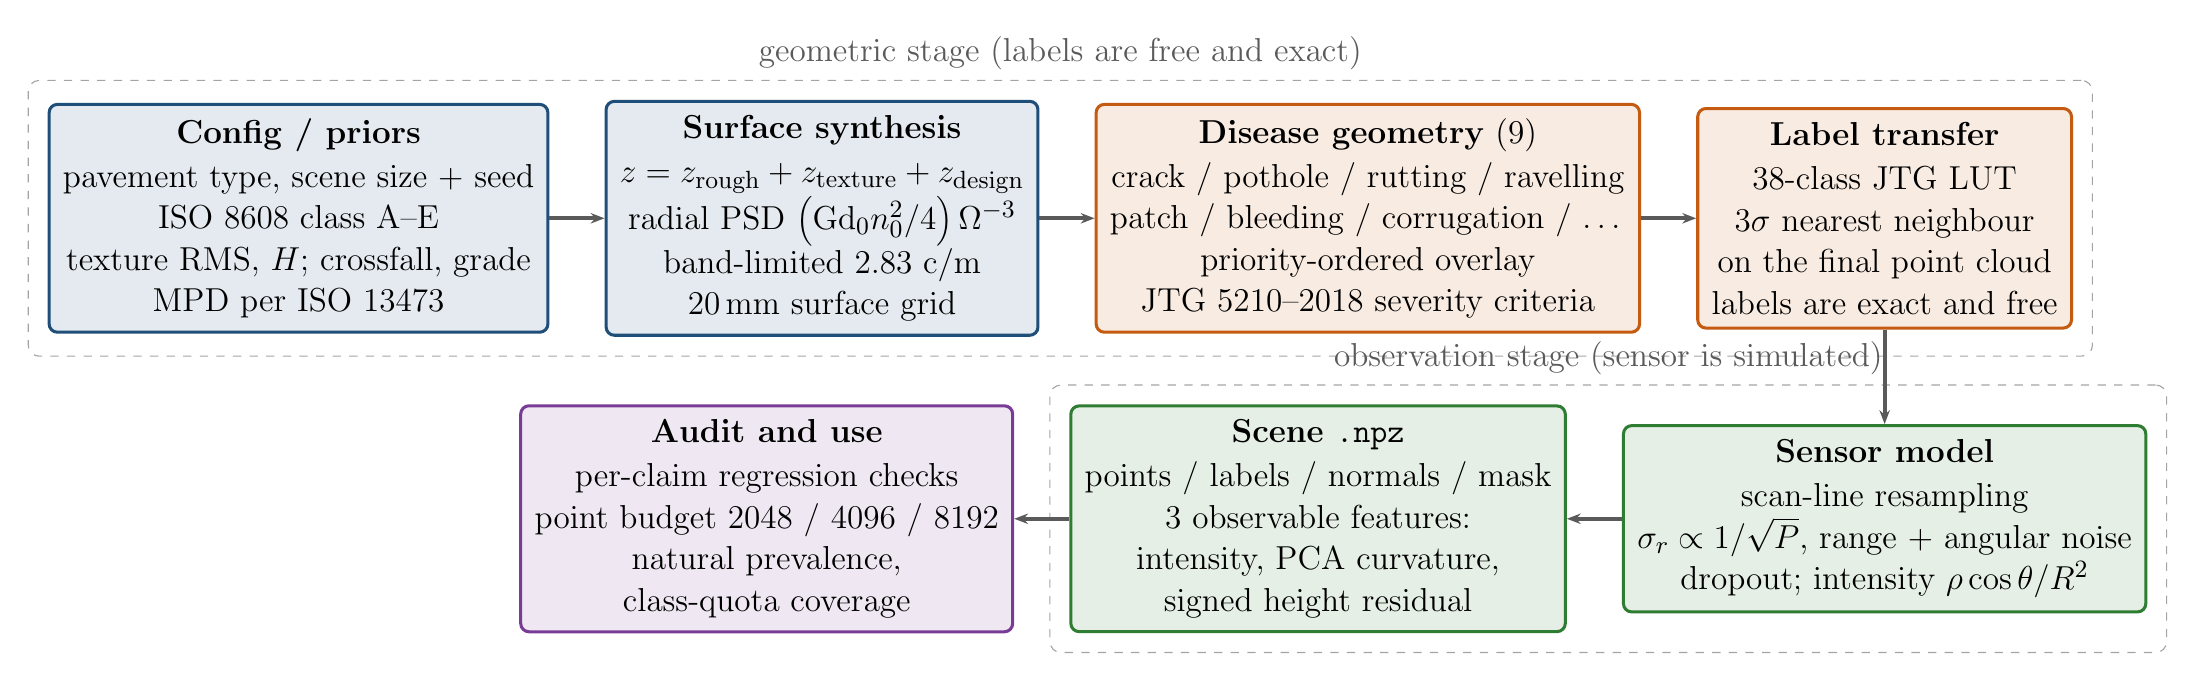
\begin{tikzpicture}[node distance=7mm and 7mm]

% ---------- 第一行：几何真值 ----------
\node[box, fill=cblue!12, draw=cblue] (cfg)
  {\textbf{Config / priors}\\[1pt] pavement type, scene size + seed\\ ISO 8608 class A--E\\ texture RMS, $H$; crossfall, grade\\ MPD per ISO 13473};

\node[box, fill=cblue!12, draw=cblue, right=of cfg] (surf)
  {\textbf{Surface synthesis}\\[1pt] $z = z_{\mathrm{rough}} + z_{\mathrm{texture}} + z_{\mathrm{design}}$\\ radial PSD $\left(\mathrm{Gd}_0 n_0^2/4\right)\Omega^{-3}$\\ band-limited $2.83\ \mathrm{c/m}$\\ 20\,mm surface grid};

\node[box, fill=camber!12, draw=camber, right=of surf] (dis)
  {\textbf{Disease geometry} (9)\\[1pt] crack / pothole / rutting / ravelling\\ patch / bleeding / corrugation / \ldots\\ priority-ordered overlay\\ JTG 5210--2018 severity criteria};

\node[box, fill=camber!12, draw=camber, right=of dis] (lab)
  {\textbf{Label transfer}\\[1pt] 38-class JTG LUT\\ $3\sigma$ nearest neighbour\\ on the final point cloud\\ labels are exact and free};

% ---------- 第二行：观测模型 ----------
\node[box, fill=cgreen!12, draw=cgreen, below=12mm of lab] (sensor)
  {\textbf{Sensor model}\\[1pt] scan-line resampling\\ $\sigma_r \propto 1/\sqrt{P}$, range + angular noise\\ dropout; intensity $\rho\cos\theta/R^{2}$};

\node[box, fill=cgreen!12, draw=cgreen, left=of sensor] (scene)
  {\textbf{Scene \texttt{.npz}}\\[1pt] points / labels / normals / mask\\ 3 observable features:\\ intensity, PCA curvature,\\ signed height residual};

\node[box, fill=cpurple!12, draw=cpurple, left=of scene] (audit)
  {\textbf{Audit and use}\\[1pt] per-claim regression checks\\ point budget 2048 / 4096 / 8192\\ natural prevalence,\\ class-quota coverage};

\draw[arr] (cfg) -- (surf);
\draw[arr] (surf) -- (dis);
\draw[arr] (dis) -- (lab);
\draw[arr] (lab) -- (sensor);
\draw[arr] (sensor) -- (scene);
\draw[arr] (scene) -- (audit);

\begin{scope}[on background layer]
  \node[grp, fit=(cfg)(surf)(dis)(lab), label={[lab]above:geometric stage (labels are free and exact)}] {};
  \node[grp, fit=(sensor)(scene), label={[lab]above:observation stage (sensor is simulated)}] {};
\end{scope}

\end{tikzpicture}
\end{document}
